{\color{gray}\hrule}
\begin{center}
\section{Théorie}
\textbf{Dans cette section, nous verrons l'aspect théorique derrière les CNNs.}
\bigskip
\end{center}
{\color{gray}\hrule}
\begin{multicols}{2}
\subsection{L'architecture}
Les CNNs se composent de deux parties principales :  
une partie dédiée à l’extraction des caractéristiques des images d’entrée, et une autre 
à leur classification.

En effet, le réseau va d'abord utiliser une couche de convolution 
pour créer des cartes de caractéristiques, puis va ensuite réduire la taille des 
données grâce à une couche de pooling. 
Ce processus est répété et ajusté selon la profondeur nécessaire au réseau.

Ensuite, les cartes de caractéristiques sont transformées en vecteurs aplatis, 
où chaque pixel devient une caractéristique. Ces vecteurs alimentent un perceptron
multicouche, qui, via des couches entièrement connectées, détermine la classe de 
chaque image.

Pour imager, nous pouvons prendre comme exemple l'architecture de la Figure 1 : 


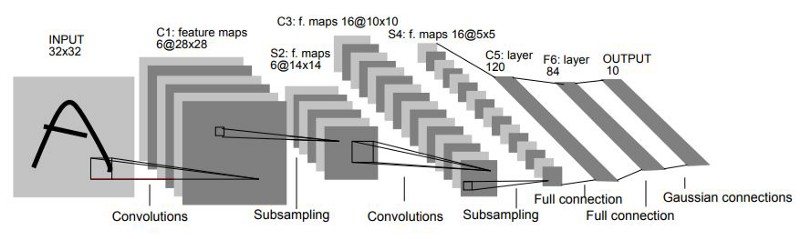
\includegraphics[width=\columnwidth]{images/lenet5.jpeg}
\captionof{figure}{Architecture de LeNet-5\cite{YannLeCunCNNs}}
\hfill\break

Nous observons deux couches de c et deux couches de pooling. On voit également le  
MLP composé d'une couche d'entrée, d'une couche cachée et d'une couche de sortie.

\subsection{Les couches de convolution}
Nous verrons ici les calculs de propagation avant et de propagation arrière nécéssaires 
à l'entrainement des couches de convolution.\\

L'opération de convolution est définie par : 

\begin{align}
y[m,n] &= x[m,n] * h[m,n]\\
&=\sum^{\infty }_{j=-\infty}\sum^{\infty }_{i=-\infty}x[i,j]h[m-i,n-j]
\end{align}
Avec $x$ l'entrée, $y$ la sortie et $h$ le filtre.\\

Cependant, pour simplifier les calculs, nous éffectuerons des opérations de cross-corrélation, définis par : 

\begin{align}
    y[m,n] &= x[m,n] \star h[m,n]\\
    &=\sum^{\infty }_{j=-\infty}\sum^{\infty }_{i=-\infty}x[i,j]h[m+i,n+j]\\
    &= \sum^{\infty }_{j=-\infty}\sum^{\infty }_{i=-\infty}x[i,j] rot_{\ang{180}}\big[h[m-i,n-j]\big] \\
    &= x[m,n] * rot_{\ang{180}} \big[h[m,n]\big] 
\end{align}

Pour nos calculs, nous posons les termes suivant : \\

$l$ l'indice d'une couche\\
$y$ la sortie\\
$x$ l'entrée\\
$w$ le filtre (ou kernel) \\
$\phi$ la fonction d'activation\\
$L$ la fonction coût\\
$m,n$ les indices des pixels de la sortie\\
$i,j$ les indices des pixels du filtre\\
$m',n'$ les indices des pixels de la dérivée de l'entrée\\
$i',j'$ les indices des pixels de la dérivée du filtre\\
$H,W$ la hauteur et la largeur de la sortie\\
$k$ la taille du filtre \\

Afin de simplifier les calculs théoriques, nous nous restreignons à une 
cross-corrélation sans padding et sur qu'un seul canal. \\

\subsubsection{Propagation Avant}

Une couche de convolution aura comme opération
en propagation avant : 

\begin{align}
y^{l} &= \phi (y^{l-1})\star w^{l} \\
&=x^{l}\star w^{l} \\
y_{m,n}^{l} &= \sum_{j=0}^{k-1}\sum_{i=0}^{k-1}\phi(y_{i,j}^{l-1}) \cdot w_{m+i,n+j}^{l}\\
&= \sum_{j=0}^{k-1}\sum_{i=0}^{k-1}\phi(y_{m+i, n+j}^{l-1}) \cdot w_{i,j}^{l}
\end{align}

Cela génère des cartes de caractéristiques qui mettent en évidence certains 
motifs d’une image, aidant le MLP à la classifier. Le nombre de cartes 
correspond au nombre de filtres dans la couche. Par exemple, pour obtenir 6 cartes 
de caractéristiques, il faut utiliser 6 filtres différents.\\

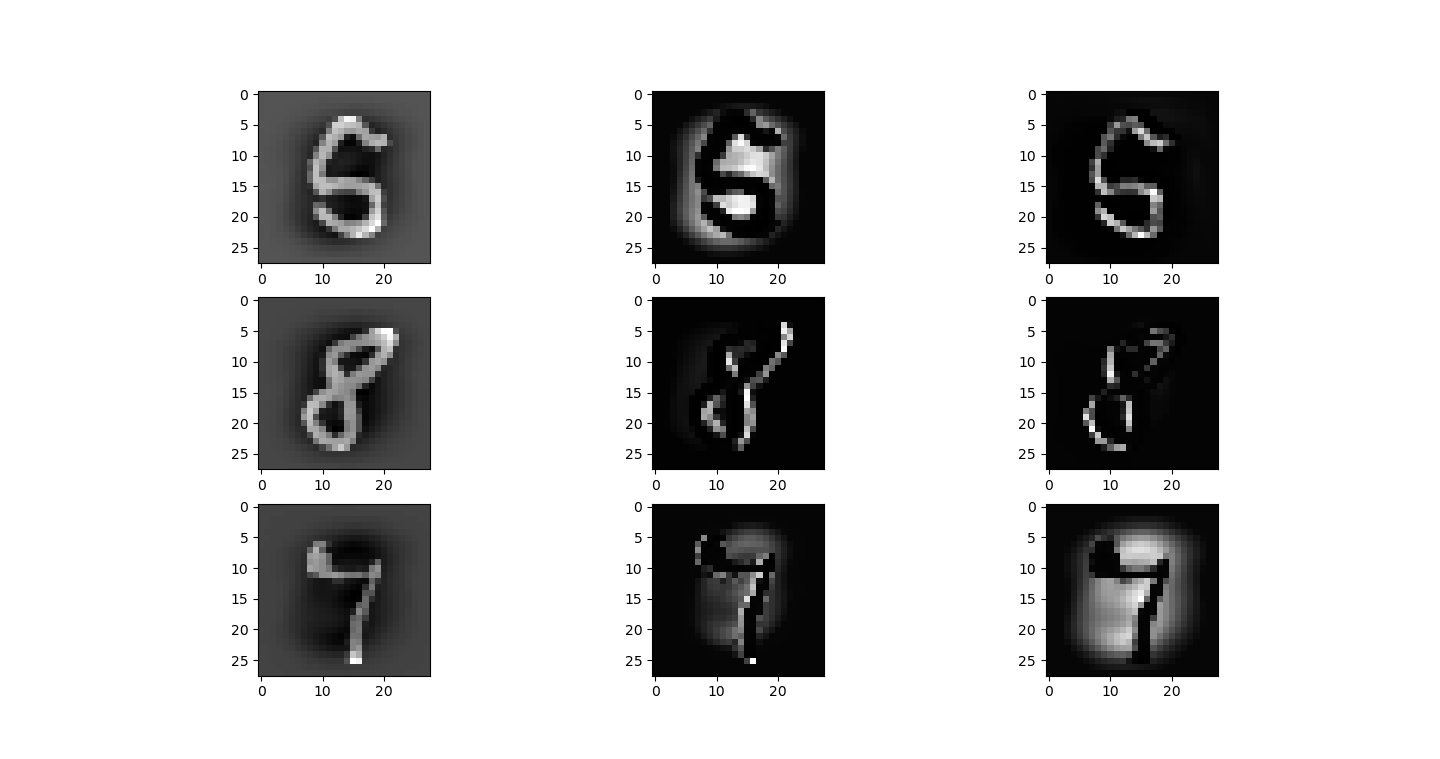
\includegraphics[width=\columnwidth]{images/featuremaps.png}
\captionof{figure}{Cartes de caractéristiques générées avec Melpy sur le dataset MNIST. 
Les entrées se situent dans la première colonne.}
\hfill\break

Sur la Figure 2, nous observons que certains pixels de l'image d'entrées sont
activés et d'autres non. On peut l'expliquer par le fait que les filtres 
vont être entrainés à activer uniquement certaines caractéristiques telles
que les bords verticaux, les bords horizontaux ou des formes plus complexes si nécessaire.\\


\subsubsection{Propagation Arrière}

En propagation arrière, nous aurons besoin des dérivées de la fonction coût $L$
par rapport à l'entrée $x^{l}$ et par rapport au filtre $w^{l}$.\\

Commençons par calculer $\frac{\partial L}{\partial w_{i',j'}^{l}}$ : 

{\scriptsize
\begin{align}
\frac{\partial L}{\partial w_{i',j'}^{l}} = \sum_{n=0}^{W-1}\sum_{m=0}^{H-1}\frac{\partial L}{\partial w_{i',j'}^{l}}\cdot\frac{\partial x_{m,n}^{l+1}}{\partial x_{m,n}^{l+1}}\\
= \sum_{n=0}^{W-1}\sum_{m=0}^{H-1}\frac{\partial L}{\partial x_{m,n}^{l+1}}\cdot\frac{\partial x_{m,n}^{l+1}}{\partial w_{i',j'}^{l}}
\end{align}}

On pose : 

$\frac{\partial{L}}{\partial{x_{m,n}^{l+1}}} = \delta^{l+1}_{m,n}$

{\scriptsize
\begin{align}
\implies \frac{\partial L}{\partial w_{i',j'}^{l}} &=  \sum_{n=0}^{W-1}\sum_{m=0}^{H-1}\delta^{l+1}_{m,n}\cdot\frac{\partial x_{m,n}^{l+1}}{\partial w_{i',j'}^{l}}\\
\frac{\partial x_{m,n}^{l+1}}{\partial w_{i',j'}^{l}}&= \frac{\partial}{\partial w_{i',j'}^{l}}\left(\sum_{j=0}^{W-1}\sum_{i=0}^{H-1}\phi(x^{l}_{m+i, n+j}) \cdot w^{l}_{i,j}\right)\\
&= \frac{\partial}{\partial w^{l}_{i',j'}}\big (\phi(x^{l}_{m+i', n+j'}) \cdot w^{l}_{i',j'}\big )\\
&= \phi(x^{l}_{m+i', n+j'}) \cdot \frac{\partial}{\partial w^{l}_{i',j'}}\big (w^{l}_{i',j'}\big )\\
&= \phi(x^{l}_{m+i',n+j'})\\
\implies \frac{\partial L}{\partial w_{i',j'}^{l}} &=  \sum_{n=0}^{W-1}\sum_{m=0}^{H-1}\delta^{l+1}_{m,n}\cdot\phi(x^{l}_{m+i',n+j'})\\
&= \delta^{l+1}_{i',j'} \star \phi(x^{l}_{i',j'})
\end{align}}

Calculons ensuite $\frac{\partial L}{\partial\phi\left(x^{l}_{m',n'}\right)}$ : 

{\scriptsize
\begin{align}
\frac{\partial L}{\partial\phi\left(x^{l}_{m',n'}\right)} &= \sum_{j=0}^{k-1}\sum_{i=0}^{k-1}\frac{\partial L}{\partial\phi\left(x^{l}_{m',n'}\right)}\cdot\frac{\partial x_{m'-i,n'-j}^{l+1}}{\partial x_{m'-i,n'-j}^{l+1}}\\
&= \sum_{j=0}^{k-1}\sum_{i=0}^{k-1}\frac{\partial L}{\partial x_{m'-i,n'-j}^{l+1}}\cdot\frac{\partial x_{m'-i,n'-j}^{l+1}}{\partial\phi\left(x^{l}_{m',n'}\right)}\\
&=   \sum_{j=0}^{k-1}\sum_{i=0}^{k-1}\delta^{l+1}_{m'-i,n'-j}\cdot\frac{\partial x_{m'-i,n'-j}^{l+1}}{\partial\phi\left(x^{l}_{m',n'}\right)}\\
\begin{split}
    \frac{\partial x_{m'-i,n'-j}^{l+1}}{\partial\phi\left(x^{l}_{m',n'}\right)} &= \frac{\partial}{\partial\phi\left(x^{l}_{m',n'}\right)}\left( \sum_{j'=0}^{k-1}\sum_{i'=0}^{k-1}\right.  \\ 
    &  \biggl.\phi(x^{l}_{m'-i+i',n'-j+j'})  \cdot w^{l}_{i',j'}  \bigg)
\end{split} \\
&= \frac{\partial}{\partial\phi\left(x^{l}_{m',n'}\right)}\big(\phi(x^{l}_{m',n'})\cdot w^{l}_{i,j}\big)\\
&= w^{l}_{i,j}\cdot \frac{\partial}{\partial\phi\left(x^{l}_{m',n'}\right)}\big(\phi(x^{l}_{m',n'})\big)\\
&= w^{l}_{i,j}\\
\implies \frac{\partial L}{\partial\phi(x^{l}_{m',n'})} &=  \sum_{j=0}^{k-1}\sum_{i=0}^{k-1}\delta^{l+1}_{m'-i,n'-j}\cdot w^{l}_{i,j}\\
&= rot_{\ang{180}}\left \{ \sum_{j=0}^{k-1}\sum_{i=0}^{k-1}\delta^{l+1}_{m'+i,n'+j}\cdot w^{l}_{i,j} \right \} \\
& = \delta^{l+1}_{m',n'} \star rot_{\ang{180}}\{w^{l}_{m',n'}\}
\end{align}}

\textit{Lors du calcul de $\frac{\partial L}{\partial\phi\left(x^{l}_{m',n'}\right)}$, nous avons éffectué une convolution. 
Cela vient du fait que les éléments de la dérivée doivent être positionnés à l'emplacement des pixels 
ayant contribué aux erreurs correspondantes.}\\

Les dérivées calculées sont ensuite utilisées dans un algorithme de Descente de Gradient\cite{GradientDescent},
afin de mettre à jour le reste des paramètres du réseau.

\subsection{Les couches de pooling}
Une couche de pooling résume les informations d’une image en réduisant les pixels 
d’une fenêtre à une seule valeur représentative. Cette méthode, déjà présente en 1998 dans l'architecture de 
LeNet-5, réduit également le coût des calculs en temps et en mémoire. Nous étudierons 
ici l’une de ses variantes les plus courantes :  le max pooling. 

\subsubsection{Propagation Avant}

Le pooling est une opération algorithmique donc nous n'aborderons pas
la formulation mathématique.\\

Deux paramètres influencent le max pooling : le \textit{stride} et 
la taille de la fenêtre (\textit{poolsize}). Le \textit{stride} détermine 
le nombre de pixels à sauter entre chaque position de la fenêtre.

Cette dernière de taille \textit{poolsize} parcourt les pixels en lignes 
et en colonnes, avec un pas de valeur \textit{stride}, pour produire une nouvelle 
image de taille $\lfloor \frac{Taille \ d’entr \acute{e}e - Poolsize}{Stride} + 1 \rfloor$. 
À chaque déplacement, elle sélectionne la valeur maximale de la fenêtre 
analysée, constituant un nouveau pixel de la sortie.\\

On peut visualiser l'opération de la manière suivante : \\

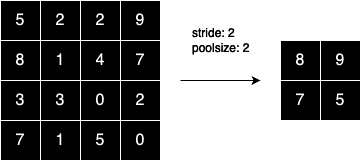
\includegraphics[width=\columnwidth]{images/forwardpooling.png}
\captionof{figure}{Exemple de la propagation avant d'un max pooling}
\hfill\break

Dans la Figure 3, nous voyons qu'un max pooling de \textit{poolsize} 2 et 
de \textit{stride} 2 a eu pour effet de diviser la taille de l'image par 2.\\

Sur une image réelle, l'opération donnerait le résultat suivant : \\

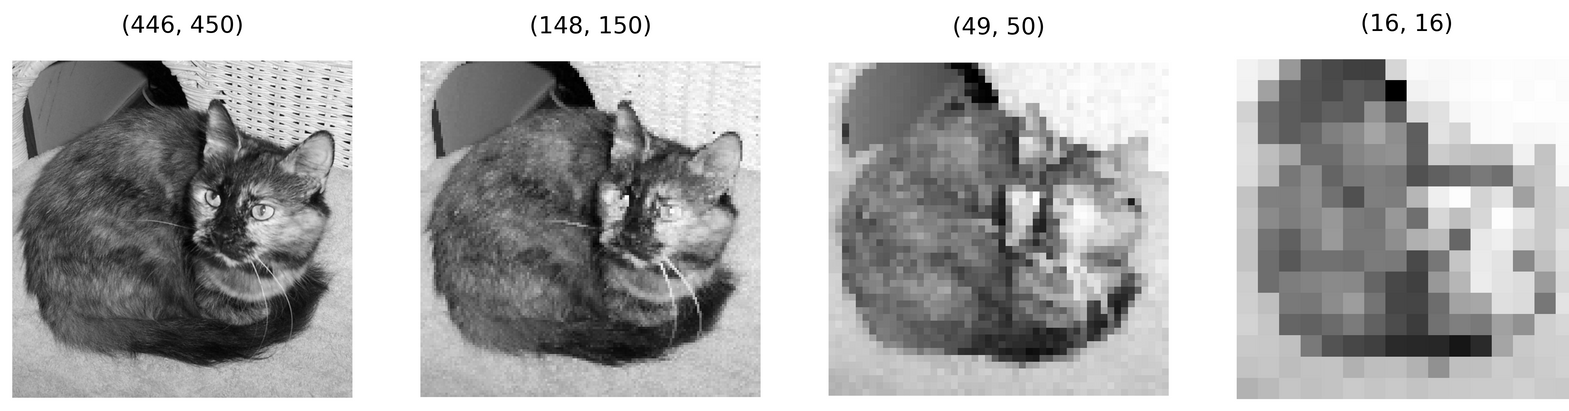
\includegraphics[width=\columnwidth]{images/maxpooling2.png}
\captionof{figure}{Exemple d'une opération de max pooling sur une image\cite{maxpoolingImage2}}
\hfill\break

On observe ici une réduction de la taille de l’image tout en préservant ses 
informations essentielles.

\subsubsection{Propagation Arrière}

En propagation arrière, on redistribue les erreurs de la couche précédente, aux positions des
maxima utilisé en propagation avant. Les autres pixels sont quant à eux désactivés. \\

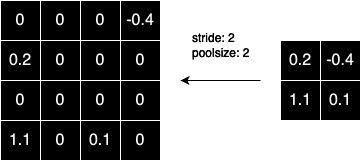
\includegraphics[width=\columnwidth]{images/backwardpooling.png}
\captionof{figure}{Exemple de la propagation arrière d'un max pooling}
\hfill\break

\end{multicols}